% =====================================================================
% Modelling-workflow schematic for the epidemic-control study.
% Self-contained: compiles with pdflatex as-is.
% Built on top of the provided neutral skeleton (node + directed arrow).
% =====================================================================
\documentclass{article}
\usepackage[margin=1in]{geometry}
\usepackage{tikz}
\usetikzlibrary{positioning,shapes.geometric,arrows.meta,calc}

\begin{document}
\pagestyle{empty}

\begin{figure}[htbp]
\centering
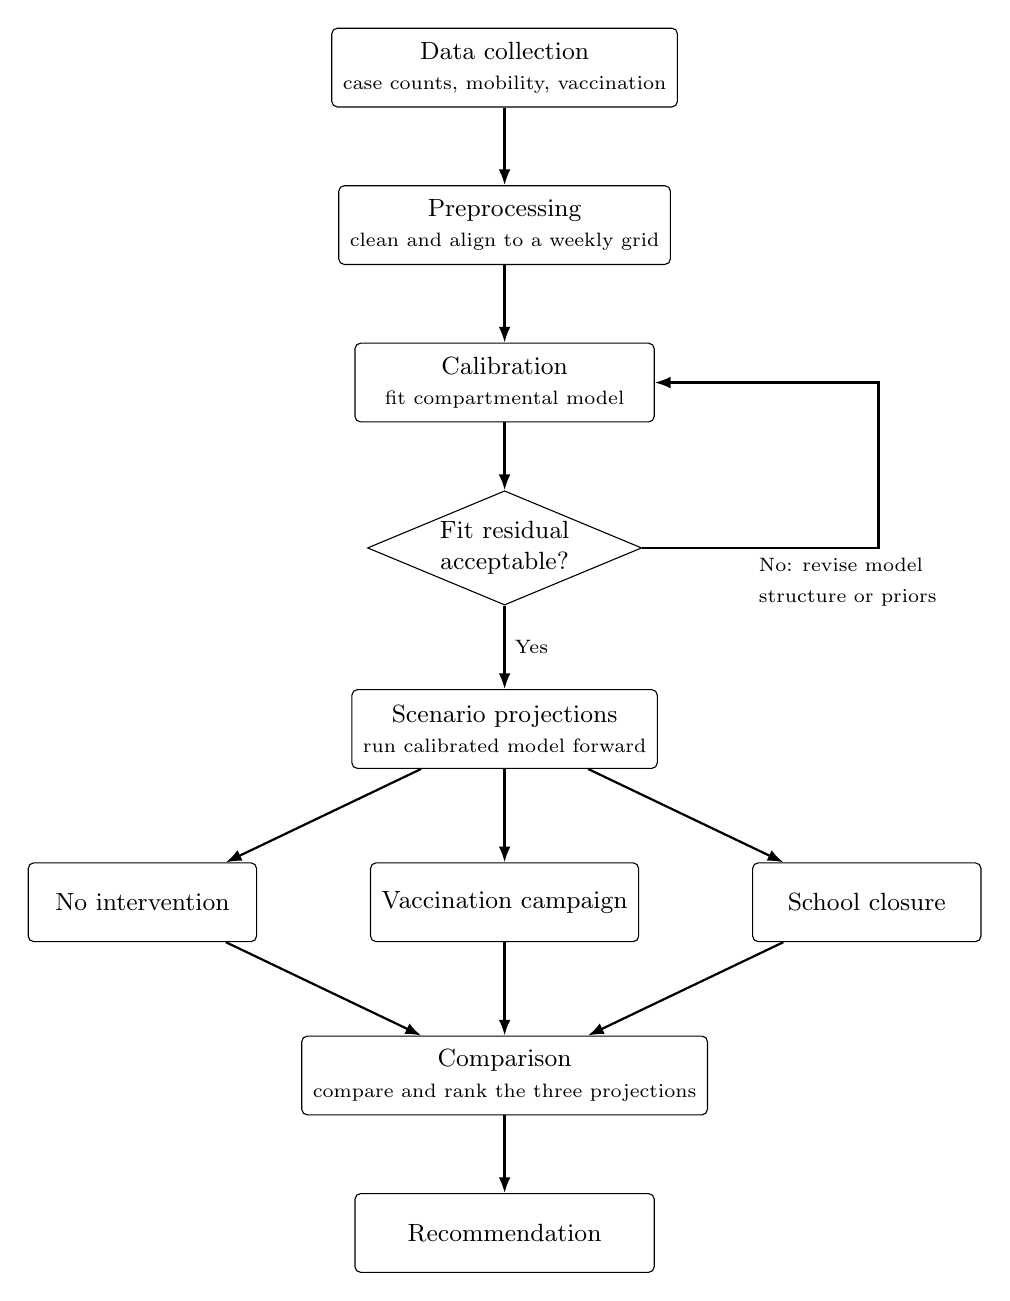
\begin{tikzpicture}[
  every node/.style={font=\small},
  proc/.style={draw, rounded corners=2pt, align=center,
               minimum width=3.8cm, minimum height=1.0cm, inner sep=4pt},
  decision/.style={draw, diamond, aspect=2.4, align=center,
                   inner sep=1pt, minimum width=3.4cm},
  branch/.style={draw, rounded corners=2pt, align=center,
                 minimum width=2.9cm, minimum height=1.0cm, inner sep=4pt},
  arrow/.style={-{Latex[length=2mm]}, thick},
  flow/.style={arrow},
]

% ---- main column -----------------------------------------------------
\node[proc] (data) at (0,0)          {Data collection\\{\scriptsize case counts, mobility, vaccination}};
\node[proc] (prep) at (0,-2.0)       {Preprocessing\\{\scriptsize clean and align to a weekly grid}};
\node[proc] (calib) at (0,-4.0)      {Calibration\\{\scriptsize fit compartmental model}};
\node[decision] (fit) at (0,-6.1)    {Fit residual\\acceptable?};
\node[proc] (proj) at (0,-8.4)       {Scenario projections\\{\scriptsize run calibrated model forward}};

% ---- three policy branches ------------------------------------------
\node[branch] (polA) at (-4.6,-10.6) {No intervention};
\node[branch] (polB) at (0,-10.6)    {Vaccination campaign};
\node[branch] (polC) at (4.6,-10.6)  {School closure};

% ---- convergence and output -----------------------------------------
\node[proc] (comp) at (0,-12.8)      {Comparison\\{\scriptsize compare and rank the three projections}};
\node[proc] (rec)  at (0,-14.8)      {Recommendation};

% ---- forward flow ----------------------------------------------------
\draw[flow] (data) -- (prep);
\draw[flow] (prep) -- (calib);
\draw[flow] (calib) -- (fit);
\draw[flow] (fit) -- node[right, pos=0.5] {\scriptsize Yes} (proj);

\draw[flow] (proj) -- (polA);
\draw[flow] (proj) -- (polB);
\draw[flow] (proj) -- (polC);

\draw[flow] (polA) -- (comp);
\draw[flow] (polB) -- (comp);
\draw[flow] (polC) -- (comp);

\draw[flow] (comp) -- (rec);

% ---- feedback loop: fit check -> calibration -------------------------
\draw[flow] (fit.east) -- ++(3.0,0)
      node[below right, pos=0.45, align=left] {\scriptsize No: revise model\\\scriptsize structure or priors}
      |- (calib.east);

\end{tikzpicture}
\caption{Modelling workflow. Weekly case counts, mobility traces and
vaccination coverage for the study city are collected and, during
preprocessing, cleaned and aligned onto a common weekly grid.
Transmission parameters are then estimated by fitting a compartmental
model to the aligned data. If the fit residual is not acceptable, the
model structure or the priors are revised and calibration is repeated
(this loop may run more than once). Once the fit is acceptable, the
calibrated model is projected forward under three alternative policies
--- no intervention, a vaccination campaign, and school closure --- and
the three projections are compared and ranked to produce the
recommendation written into the paper.}
\end{figure}

\end{document}
